\chapter{Used Technology Analysis} \label{chap:2}
    \epigraph{If I have seen farther than others, it is because I was standing on the shoulders of giants.}{\textit{Isaac Newton}}

    According to the discussion in the previous chapter we have settled on docker containers running Ubuntu for providing the backbone of our virtualized networks. This section is concerned with analyzing the different technologies that will play a role in supporting the virtual network infrastructures we are to create.\\

    \section{The Network Stack}
        A fascinating but rather overwhelming image can be seen on figure \ref{fig:linux-map}. If we pay close attention we will see how one of its columns is just devoted to networking. The software entities comprising this column is what we will refer to as \textit{Linux's Network Stack}\\

        \begin{figure}
            \centering
            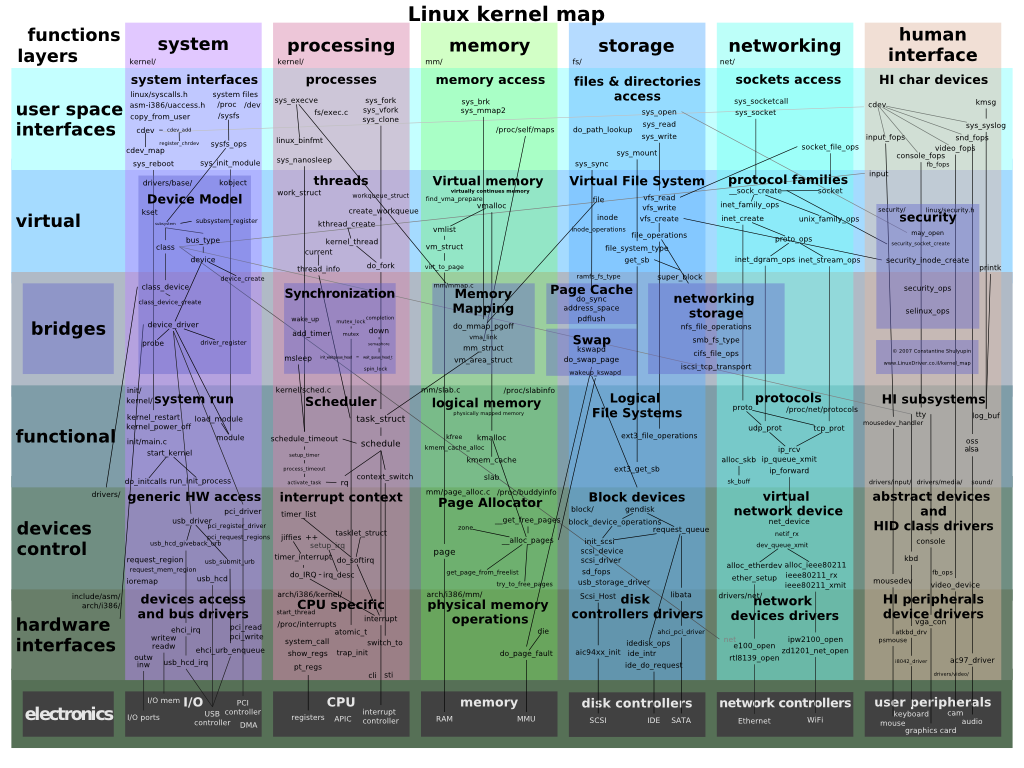
\includegraphics[width=0.5\linewidth]{linux_map.png}
            \caption[Linux Kernel Structure]{Linux's ``Map''. \cite{bib:linux-map}}
            \label{fig:linux-map}
        \end{figure}

         The word stack is something that shows up time and time again in the area of networking. It helps us have a top-level view of how logical entities cooperate within a network. When we think about stacks we naturally begin to consider them in terms of the layers they are composed by, with each layer tackling a simple task and offering services to the layer above whilst using those provided by the layer below. It is not going to be any different with Linux; we can think of its network stack as a huge ``blob'' of code which all network packets reaching a Linux-based system traverse. Thus, if we can alter how Linux processes packets or build \textit{virtual} connections between different network stacks we would be capable of constructing a de-facto virtual network tailored to our needs.\\

         \paragraph{Naming Packets}
            Before we go on we need to shed some light on the naming we are going to use regarding the units of data exchanged through network links. Even though the term packet is tremendously generic we feel it is not a wrong one to turn to in our case. When we wire up several network nodes together we are looking for full connectivity, that is, connectivity at the application level. Thus, we are not really that interested on what layer the ``packet'' is at, we do not really care if the packet is a \texttt{segment}, \texttt{datagram} or \texttt{frame}. In the case a need for more specific naming arises, we will not hesitate to do so, but we prefer to keep the writing simple and avoid getting bogged down with technicalities whose benefit we feel is not that obvious.\\

            A prime example of the above would be the use of the term \texttt{packet} instead of \texttt{link-layer frame} in the section's introduction. \textit{Frame} is the correct term for referring to the data structure a \texttt{NIC} (Network Interface Card) hands to the kernel (albeit somewhat processed as the preamble and Frame Check Sequence of Ethernet frames are usually stripped from incoming frames by the \textit{NIC} itself as seen on \textit{WireShark's} documentation \cite{bib:wireshark-eth-doc}).\\

        If we think about network stacks, we would probably believe we need to have one per machine. That is, every network-capable devices must have their own \textit{data-path} which packets are to traverse. What may not be so simple is thinking that a machine \textit{may} have more than one network stack. In order to get a firmer grasp on the implications of the above idea let us revisit the concept of a network interface.\\

        When we first started learning about network architectures we where flabbergasted by the fact that a machine could have more than one NIC. This implied it had several different IP addresses ``attached'' to it, which provided redundancy amongst other several capabilities like traffic control. What astonished us the most was the raw power of not imposing a limit on the number of NICs a machine could have. That simple fact allowed routers to exist, for instance, and you could do seemingly useless stuff such as getting a packet through an interface and \texttt{echoing} it out the other. All in all, it provided a ton of flexibility to the whole system.\\

        Now, if we apply the above to the concept of network stacks we could be talking about packets being interchanged in between them whilst residing on the same machine nonetheless. If we sit back and take a look at the larger picture, we can clearly see that packet below the application level are logically switched between network stacks belonging to different machines as it is the stack who is in charge of processing said data structures. Seeing matters in that light, and knowing we can have several network stacks on a single platform, talking about packets being interchanged within a machine does not seem that far fetched now.\\

        Given the previous discussion we can now clearly see the base on which everything else is built upon. The ability to have several coexisting network stacks on a machine, as well as being able to connect them as we please, is such a powerful tool that our work is only scratching the surface of the capabilities enabled by this kind of technology. Linux's network stacks are nothing short of an ode to code modularity.\\

        All the previous discussion is related with the theoretical or conceptual realm of matters. We will now delve into how we can translate these ideas into a working virtual network. After going through that process we will also look into why we decided to do everything manually once we have a broader technical background on the subject.\\

        Finally, we feel we need to clarify that, even though it may be clear at this point, all the network traffic we are to generate originates from within our own system. In other words, our network would be perfectly capable of working without any Internet access.\\

    \section{The Network Namespace}
        Many of the programming languages dominating today's market are object oriented. This, very roughly, means that the programmer is expected to generate \texttt{classes} representing ``real-life'' entities to some extent. These classes are defined by their \texttt{attributes} (characteristics) and their \texttt{methods} (what they can do). Now, a class by itself cannot do anything, we need to \texttt{instantiate} it so that we create an \texttt{object} of that class. We'll then be capable of using the newly created object as we please.\\

        This concept of instantiation is actually quite powerful as it appears continuously in many areas of engineering. Now, we could say that Linux's network namespaces work in a similar fashion to classes. We can think of the network stack as the class and what we call \textit{network namespaces} as the objects.\\

        As seen on \cite{bib:man-namespaces}, namespaces are not only seen when dealing with networking, they are a feature of the Linux kernel employed in many other areas. These namespaces let us partition kernel resources so that each process sees a resource that is only for it, it is not shared. When applied to networking, we can see how each network namespace \cite{bib:man-netns} represents an entire network stack. Then, if we set up several network namespaces (namespaces from now on as this is the only type of namespace we will deal with) we have effectively housed several network stacks within the same machine. We then need to look into how we can interconnect them.\\

        Our system will model a network-capable machine as a simple process with its very own network namespace. This sentence can be quite abstract. That is why we believe a more concrete example can help the reader grasp what we are trying to entail.\\

        \subsection{A common \texttt{HTTP} server}
            The \texttt{Internet} has revolutionized society in ways little people could have predicted. It supports many different application protocols such as \texttt{SMTP} and \texttt{FTP}, but one of the most popular (if not the most) is \texttt{HTTP(S)}. This protocol provides the backbone for websites and many other applications that are employed by huge amounts of people on a daily basis.\\

            Like many other protocols, \texttt{HTTP(S)} leverages the \textit{client-server} architecture. The client role is usually ``played'' by web browsers such as \texttt{Firefox} or \texttt{Safari}, whilst the server part is relegated to programs such as \texttt{Apache} and \texttt{Nginx}. From a networking point of view, a process is univocally addressed through an \texttt{IP address} and a \texttt{port number}. The former identifies a given machine within a network whilst the latter targets a process running within that machine. Then, we can have different servers running on a \textit{physical} machine as long as their port numbers differ. We begin to see how, from a strict networking point of view, we can have several \textit{logical} entities supported by a single \textit{physical} one.\\

            Now, imagine that we want or need to run two \texttt{HTTP(S)} servers on a single machine and a single port number. That would not be possible, would it? Now, if we leverage the concept of the network namespace we can circumvent this limitation. We could, for example, instantiate two different namespaces for each of the server processes and then bind each of them to the same port \textbf{within the respective namespaces}. Then, a network-aware process together with its own network namespace is, in a way, a full-fledged logical entity within a network: it is addressed by its own \texttt{IP address} and it has its own pool of independent \texttt{port numbers}. This is exactly what our framework exploits: each virtual host is a simple process running within its very own namespace.\\

        The above was one of the main reasons we vouched for \textit{containers} as a technology before. Each container ships with its own network namespace when it comes to networking. Whilst it is true that \textit{docker} does bring up some network infrastructure with a new container, we can explicitly avoid that to be given a ``pure'' namespace with each new container. We can then manually instantiate any other network elements we might need to complete the network topology we are to build.\\

        Managing namespaces and instantiating the virtual network elements, such as \texttt{veths}, gluing them together is attainable with the help of the \texttt{iproute2} suite of tools. We will then look into how to leverage \texttt{iproute2} for our needs.\\

    \section{The \texttt{iproute2} suite}
        The time we spend on terminal emulators has exponentially increased as we worked our way through our bachelor's. Even though they provide quite a fast way to ``get around'' the computer they can be a little abstract at times. We are always aware that the OS ``under'' us has many running processes and provides us with services that can be used at our request. Nonetheless, it is crucial to leverage the help of programs that can query and show the system's status when required. This is the case for programs like \texttt{ps}, which reports the status of the system's processes, or \texttt{w}, which tells us about who is currently logged into the system as well as what they are up to. When using a shell we are aware of the fact that other processes are running and that other users may be logged in but we nonetheless have tools that let us consult the current status of the system.\\

        Where networking is concerned, \texttt{iproute2} \cite{bib:man-ip} is like a ``Swiss Army Knife''. It is a \textit{suite} or collection of tools that lets us do everything from inspecting the current interfaces and routes to generating \texttt{IPv6/IPv4} tunnels. We will only be concerned with the \texttt{ip} command in our case which is in charge of \textit{``showing/manipulating routing tables, network devices, interfaces and tunnels''} as seen in \texttt{ip}'s manpage (which can be consulted with \texttt{man ip}). The uses one can give to \texttt{iproute2} are seemingly endless, but before getting into them we believe it would be useful to compare the \texttt{iproute2} suite to its predecessor: \texttt{net-tools}.\\

        \subsection{The deprecated solution: \texttt{ifconfig}}
            Querying a system's interfaces is a very common task in the day of a network engineer. Whenever Internet connectivity is not behaving as expected or network connections do not seem to be working as intended, our initial step is to check interfaces are configured as they should. On \texttt{Unix}-based systems such as \texttt{macOS} and \texttt{GUN/Linux} this was traditionally accomplished with the \texttt{ifconfig} command. Before \texttt{iproute2} was implemented, network-related tools fulfilling the same purpose were provided by the \texttt{net-tools} suite. Among the most well-known tools provided by it we can mention \texttt{ifconfig} and \texttt{netstat}. The former displayed information on the system's network interfaces whilst the latter shed light on the open sockets in the system. When working with network-centric applications such as web-servers, \texttt{netstat} was a superb way of finding out whether some process had \texttt{binded} (i.e. began listening) to the \texttt{80} or \texttt{443} ports, each being the default for the \texttt{HTTP} and \texttt{HTTPS} protocols, respectively. With time, \texttt{iproute2} became available and it \textit{deprecated} \cite{bib:net-tools-deprecation} the \texttt{net-tools} suite. We have nonetheless observed throughout our studies that a non-negligible amount of people are reluctant to abandon \texttt{ifconfig} and related tools.\\

            What we are trying to achieve with this project is possible if leveraging \texttt{net-tools} instead of \texttt{iproute2}. However, the former's documentation and examples tend to be more cryptic and harder to digest. What is more, even though people resist to stop using it, \texttt{net-tools} is bound to disappear. That is why using the newer network tools confers a longer life prospect to our work.\\

            Even though \texttt{net-tools} has been deprecated on \texttt{linux-based} systems, it's still the selected network tool suite for systems such as \texttt{macOS} where \texttt{iproute2} is \textbf{not available}. Some programs such as \texttt{iproute2mac} do exist for this operating system, but they just \textit{parse} (i.e. process) the output provided by \texttt{net-tools} utilities and present it following \texttt{iproute2}'s format. We must not be deceived by looks: \texttt{iproute2} is a part of \textbf{\texttt{linux}} systems. We compare both suites on table \ref{tab:net-tools-vs-iproute2}.\\

            \begin{table}
                \centering
                \begin{tabular}{|c|c|}
                    \hline
                    \textbf{net-tools} & \textbf{iproute2}\\
                    \hline
                    \texttt{arp} & \texttt{ip neigh}\\
                    \hline
                    \texttt{ifconfig} & \texttt{ip addr}, \texttt{ip link}, \texttt{ip tunnel}\\
                    \hline
                    \texttt{netstat} & \texttt{ss}, \texttt{ip maddr}\\
                    \hline
                    \texttt{route} & \texttt{ip route}\\
                    \hline
                \end{tabular}
                \caption[\textit{net-tools} vs. \textit{iproute2}]{\textit{net-tools} utils vs. \textit{iproute2's}. \cite{bib:nettools-vs-iproute2}}
                \label{tab:net-tools-vs-iproute2}
            \end{table}

        \subsection{Describing a network interface}
            In a previous section we already provided some comments on what NICs are. Knowing that interfaces create ``bridges'' between different systems we can clearly see how these network interfaces connect digital systems to a communication network; they let these digital machines leverage the communication capacities of computer networks.\\

            Whilst almost all engineers could recognize what a NIC physically is, the matter is not that simple regarding how the OS treats these interfaces. We find it quite helpful to think of what we would do if we had to implement some software solutions that had to employ the network's capabilities. There must be a ``way'' that these hardware components can be used from the application perspective, that is, the OS needs to offer some kind of abstraction through which we can use the NIC itself. This abstraction is what we will call a OS-level NIC or network interface. Then, applications need only be concerned with opening \texttt{sockets} that are then supported by one of the system's network interfaces.\\

        Knowing a bit about what \texttt{iproute2} is, we believe walking through some examples showing how to instantiate virtual network elements will prove rather revealing.\\

    \section{Instantiating virtual network elements}
        As \texttt{iproute2} offers us total control over a machine's internal network infrastructure, we believe the best way to showcase what we can do is through example. Before getting down to the ``command level'' of matters, let us establish some naming conventions.\\

        \subsection{Naming network elements}
            The networks we will work with are rather simple when it comes to the type of elements they are composed of. Even though they can grow quite large, from a network architecture point of view they will reuse the same components over and over. These components are:\\

            \begin{itemize}
                \item \textbf{\texttt{Link-level bridges}:} These \textit{layer 2} devices will forward \textit{link-layer frames} within a subnetwork based on the destination \texttt{MAC address}. These are \textbf{transparent} to \textit{layer 3} (i.e. \textit{network}) protocols such as \texttt{IP}. These are implemented as a \texttt{linux bridge} which, in turn, manifests itself as a network interface. They'll provide the backbone for each of the subnets we are to instantiate as they provide their very own broadcast domain. One can find documentation regarding these bridges on \cite{bib:kernel-brds}.

                \item \textbf{\texttt{Network-level routers} and \texttt{firewalls}:} These \textit{layer 3} devices will forward packets between subnetworks based on the destination \texttt{IP} address. These will be implemented as \texttt{containers} running a regular \texttt{Ubuntu} image with minor additions. Given these routers are located between subnetworks, we will also implement any required firewall functionality within them as well. We will delve deeper into how this can be accomplished in due time, but we can already say that these firewalls are based on \texttt{iptables}.

                \item \textbf{\texttt{End hosts}:} These are the end systems in the network. They'll be implemented as \texttt{docker containers} running a lightly modified Ubuntu image as well.

                \item \textbf{\texttt{Veths}:} These are \textit{virtual Ethernet interfaces} which we will use to wire the entire network together. These virtual interfaces can be regarded as ``virtual wires'' with two ends. Any frame coming into one end comes out the other and vice-versa. We can then conclude they behave exactly like real-world wires. We will then ``insert'' one end of a \texttt{veth} into a network device and the other end into another one to effectively ``wire them together''.

                \item \textbf{\texttt{Network namespace}:} We would like to make it absolutely clear that \textit{namespaces} are \textbf{not} network devices per-se: they have no real world counterpart. As we will later see, each \texttt{container} spawns its own \textit{namespace}: we have a one-to-one correspondence between hosts/routers and namespaces. This will be crucial when connecting network elements with \texttt{veths}, as they will have to be associated to a particular network namespace for things to work.
            \end{itemize}

        Now that we have settled the naming scheme we will use, it is time to break down some commands allowing us to instantiate virtual network elements as we please.\\

        \subsection{\texttt{Bridges}}
            Just like we stated before, \texttt{bridges} are \textit{layer 2} devices. We will find how, due to their operation, no configuration is needed beyond bridge creation. These devices will automatically learn link-level routes as needed whilst in operation. As we are concerned with the link layer, we will be dealing with physical or \texttt{MAC} (\textbf{M}edia \textbf{A}ccess \textbf{C}ontrol) addresses. These are very characteristic in the sense that they are represented as a series of \textit{hexadecimal} digits separated in groups of $2$ by colons (\texttt{:}). Given the intricacies of a $base-16$ numbering system, each of these colon-delimited groups is equivalent to a single \textit{byte} of data. Anyhow, an example of a \texttt{MAC} address would be: \texttt{8c:2d:aa:56:e2:7b}. As a curiosity, we can indicate that different \texttt{MAC} prefixes are allocated to manufacturers by the \texttt{IEEE}. That means that we can know the manufacturer of a pice of equipment through its \texttt{MAC} address (assuming it has not been tampered with). If one were to check the above address, he or she would find it to belong to a device manufactured by \textit{Apple Inc.}. After all, it is the \texttt{MAC} of the \textit{iMac} we are writing this document on.\\

            The bottom line to the above is that a bridge's \texttt{MAC} forwarding table need not be configured explicitly, be it through a protocol or a human operator. As soon as the bridge is brought up, it'll broadcast an incoming link-layer frame on all of its interfaces but the one the frame arrived on. The key aspect here is that the bridge will include an entry in its forwarding table associating this frame's \textbf{source MAC} to the interface the frame arrived on. If that original frame's \texttt{MAC} address was, say, \texttt{01:23:45:67:89:AB} and the frame arrived on port \texttt{0}, the bridge would automatically learn to send any incoming frame with destination \texttt{MAC 01:23:45:67:89:AB} through port \texttt{0}. After being in operation for some time, the bridge will throttle back the number of frames it broadcasts, thus operating ever more efficiently. An aspect to keep in mind with this way of automatically configuring the forwarding tables is that these entries need some way of being deleted. Just like with learning, this will be an implicit process requiring no explicit signaling whatsoever. The learnt entries will be associated to a timer. When this timer runs out, the route will be assumed to be stale and be deleted from the table. This mechanism allows us to remain true to the real network topology whilst being stable enough in the face of network changes.\\

            We believe the above discussion to be relevant as a way of justifying why we need not be concerned with any configuration whatsoever. The very design of real \texttt{bridges} (and thus of its virtual counterparts) takes care of this for us. We will later see how this is not the case for network level routers. We'll need to manually populate the routing tables so that we attain the desired topology.\\

            We would also like to state that we did have to overcome a slight but hard-to-spot problem related to these bridges. It involves a setting controlling whether to involve \texttt{iptables} in frame forwarding at each of the virtual bridges. As this interaction has several important implications, such as violating a ``pure'' layered architecture we will delve deeper into it in section \ref{sec:bridge-caveats}.\\

            Even though the previous paragraphs might make bridge creation look cumbersome, it could not be any simpler. Getting a working bridge is a matter of executing the lines found on listing \ref{lst:bridge-creation} from a shell. As listing \ref{lst:bridge-creation} contains commands that ought to be run in a shell we would like to discuss the necessary execution permissions so that someone trying to recreate this work can do so in a satisfactory way.\\

            \subsubsection{Capabilities for network infrastructure handling}
                Unleashing \texttt{iproute2}'s full potential implies that we can wreck havoc on a system's network infrastructure. We could leave the entire system without network connectivity or alter the way traffic is processed in such a way that we could snoop on user's data, for example. This implies that not everybody using a system should be able to perform these actions.\\

                One of the ideas at the core of any system is \textit{access control}. It lets us control what system users can and cannot do in such a way that we protect the system's stability and security. Each user will have different capabilities to perform actions on the system. One can read on them on \texttt{manpages} such as the one provided by running \texttt{man capabilities}, but the bottom line is that not every user will be able to use all of \texttt{iproute2}'s features without them being granted some capabilities. Given the configuration overhead this entails, we opted for issuing restricted commands as the system's \texttt{root} user whose \textit{user id} (\texttt{UID}) is \texttt{0}. This implies it bypasses all capability checks: that is, \texttt{root} has unrestricted access to \texttt{iproute2}'s features. On \texttt{UNIX}-based systems one can either opt for prepending \texttt{sudo} to commands such as the ones on listing \ref{lst:bridge-creation} or just run all of them as \texttt{root} directly. The latter can be achieved by running \texttt{su -} to switch users. These are by no means the only ways of running the commands we include in this document. One can grant the required capabilities to an arbitrary user to perform the same tasks whilst being more elegant with respect to capability handling. Again, the information found on \texttt{man capabilities} is a wonderful stepping stone for more complex capability-oriented setups.\\

                We will revisit capabilities when discussing the method of creating \textit{docker containers} later down the road as it's a crucial step for enabling the management of a container's networking infrastructure.\\

            \begin{lstlisting}[language = bash, caption = Instantiating a Virtual Network Bridge., label = lst:bridge-creation]
                # Create a new virtual bridge named foo-brd.
                ip link add foo-brd type bridge

                # Bring it up (i.e. turn it on).
                ip link set foo-brd up

                # Check the bridge is indeed up.
                ip link

                # This should provide an output like the following:
                # 4: foo-brd: <BROADCAST,MULTICAST,UP,LOWER_UP>\
                    # mtu 1500 qdisc noqueue state UNKNOWN mode DEFAULT
                    # group default qlen\
                    # link/ether 72:8a:77:68:42:b1 brd ff:ff:ff:ff:ff:ff
            \end{lstlisting}

            We would like to draw the reader's attention to the \texttt{LOWER\_UP} string found on \texttt{ip link}'s output on listing \ref{lst:bridge-creation}, as it is letting us know that the newly created \texttt{bridge} is indeed active. On top of that, we would also like to note that the backslash (\texttt{\textbackslash}) characters found on \texttt{ip link}'s output are \textbf{not} present on the ``real'' output. We have included them out of necessity, given the output lines were too long to be displayed on a single line in this document. We decided to indicate where we had broken up the line in an effort to be true to the original text whilst making it more visually appealing. This small ``tweak'' has been applied on other listings such as \ref{lst:veth-creation}.\\

        \subsection{\texttt{Veths}}
            Now that we know how to create \texttt{bridges} it is time to instantiate the ``wires'' connecting all of them together \cite{bib:man-veth}. Just like we explained before, these ``wires'' are supported on \texttt{veths}. The creation process is very similar to that of bridges in the sense that we will leverage \texttt{ip link}'s functionality. Listing \ref{lst:veth-creation} shows how these \texttt{veths} are created. From \texttt{iproute2}'s perspective, these \texttt{veths} manifest as two different interfaces that are nonetheless very intimately related. Just like we explained before, everything that enters one \texttt{veth} end will go out the other and vice-versa. This relation is made clear by how these \texttt{veths} are displayed when querying the network configuration as seen on listing \ref{lst:veth-creation}.\\

            \begin{lstlisting}[language = bash, caption = Instantiating a Virtual Ethernet Interface., label = lst:veth-creation]
                # Create a new veth whose ends are named veth-end-x and
                    # veth-end-y.
                ip link add veth-end-x type veth peer name veth-end-y

                # Bring BOTH ENDS up.
                ip link set veth-end-x up
                ip link set veth-end-y up

                # Check the veth ends are indeed up.
                ip link

                # This should provide an output like the following:
                # 5: veth-end-y@veth-end-x: <BROADCAST,MULTICAST,UP,\
                    # LOWER_UP> mtu 1500 qdisc noqueue state UP mode\
                    # DEFAULT group default qlen 1000\
                    # link/ether 5e:b1:40:3f:e7:53 brd ff:ff:ff:ff:ff:ff
                # 6: veth-end-x@veth-end-y: <BROADCAST,MULTICAST,UP,\
                    # LOWER_UP> mtu 1500 qdisc noqueue state UP mode\
                    # DEFAULT group default qlen 1000\
                    # link/ether de:16:80:f6:c3:64 brd ff:ff:ff:ff:ff:ff
            \end{lstlisting}

            When looking at listing \ref{lst:veth-creation} we find that, just like in listing \ref{lst:bridge-creation}, the \texttt{LOWER\_UP} string is telling us that both \texttt{veth} ends are up and running. We would also like to bring the reader's attention to the \texttt{@veth-end-[x/y]} suffix in both \texttt{veth} names. This is just telling us the name of the other \texttt{veth} end associated with this one. In other words, \texttt{veth-end-y@veth-end-x} tells us that the \texttt{veth} whose configuration we are currently inspecting (i.e. \texttt{veth-end-y}) is attached to \texttt{veth-end-x}. Nonetheless, we need not specify this suffix when referring to the \texttt{veth} ends during configuration. Note we didn't include it on lines $5$ and $6$ on the same listing.\\

            \subsubsection{Adding \texttt{veths} to network namespaces}
                With what we have seen on the previous section we are only capable of creating the \texttt{veths} themselves. In order for them to be useful we need to somehow connect them to other network elements so that they are ``physically'' connected. The process of connecting \texttt{veth} depends on what element we are to connect it to. Even though it only takes a single command to do, the connection of \texttt{veths} is a more conceptually intricate process that requires us to recall what network namespaces were.\\

                When dealing with \texttt{bridges} we just need to issue a simple command as seen on listing \ref{lst:veth-brd-cnx}. Said instruction would be the ``virtual'' equivalent of walking up to a real \texttt{bridge} and plugging an \texttt{Ethernet} wire in, for instance.\\

                \begin{lstlisting}[language = bash, caption = Connecting a \texttt{veth} end to a virtual \texttt{bridge}., label = lst:veth-brd-cnx]
                    # Connect veth end veth-end-x to bridge foo-brd
                    ip link set veth-end-x master foo-brd
                \end{lstlisting}

                Now, connecting a \texttt{veth} to a host is a more intricate process. Even though it is true that it only requires a single command, we need be clear about the ``conceptual domain'' backing said connection up. Doing so requires recalling what \textit{network namespaces} were. In the realm of networking we stated that a network namespace could be regarded as an independent network stack within a single physical machine. Thus, each process that was granted its own would ``believe'' to have its own, independent network stack. We also teased that each of our network nodes (both hosts and routers) would run as a docker container and that each of them would have an associated namespace. Thus, connecting a \texttt{veth} to a host or router is a synonym for making said \texttt{veth} a part of that namespace. This can be accomplished through a single command as seen on listing \ref{lst:veth-namespace-cnx}. We would like to stress the fact that in order for said command to behave as expected we must ensure \texttt{iproute2} can ``see'' the namespace we are trying to add the \texttt{veth} to. This is a topic we will delve into in the following section.\\

                \begin{lstlisting}[language = bash, caption = Connecting a \texttt{veth} end to a host or router., label = lst:veth-namespace-cnx]
                    # Connect veth end veth-end-y to a host whose associated
                        # namespace is host-a-ns
                    ip link set veth-end-y netns host-a-ns
                \end{lstlisting}

        \subsection{Managing network namespaces}
            Given the framework we have designed we will need to circumvent some small limitations to leverage the \texttt{iproute2} suite. We will explained what these are and how to quench them before explaining how to work with \texttt{iproute2} in a ``multi-namespace'' setup.\\

            \subsubsection{Making \texttt{iproute2} aware of container namespaces}
                The command we presented on listing \ref{lst:veth-namespace-cnx} depends on \texttt{iproute2} being aware of the existence of the \texttt{host-a-ns} network namespace. This will not be an issue if the namespace itself is created with the same suite of tools. However, this is \textbf{not} our case: we are trying to interact with network namespaces our docker containers are managing themselves. This implies that we need to manually perform some actions to let \texttt{iproute2} manage these namespaces too.\\

                Working with virtual network infrastructure and namespaces is rather abstract. Thus, commands letting us inspect the current state of affairs are tremendously helpful. In this case we can leverage \texttt{ip netns}. This will list all the namespaces the \texttt{iproute2} suite is currently aware of (and thus, those it can currently manage and modify). If we \texttt{run} a docker container and compare the output of the \texttt{ip netns} command before and after doing so we \textbf{will not} appreciate any difference. This follows from the fact that, as we stated before, the associated namespace is managed by \texttt{docker} itself. After performing the actions we detail on the next paragraph one will be able to check how the output shown by \texttt{ip netns} does reflect the newly created namespace.\\

                The key idea to keep in mind is that ``a named network namespace is an object at \texttt{/var/run/netns/NAME} that can be opened'' as stated on \texttt{ip-netns}'s \textit{manpage}. Note that in order to be sure that we are obtaining information relevant for our platform we must make sure this \textit{manpage} is queried on a machine running \texttt{Ubuntu} or on a site offering \texttt{Ubuntu}'s \textit{manpages}. All in all, we find that in order for \texttt{iproute2} to be aware of network namespaces these must be available at \texttt{/var/run/netns}. If we create a network namespace ourselves with \texttt{ip netns add foo-ns} we would find that the \texttt{ip netns} command now shows \texttt{foo-ns} on its output and that there would be a new empty file at \texttt{/var/run/netns/foo-ns}. The latter is the ``manifestation'' of the newly created network namespace on our filesystem. As expected, \texttt{running} a \texttt{docker} container \textbf{does not} place any file under \texttt{/var/run/netns} and so \texttt{iproute2} cannot manage that namespace. Nonetheless, the fact that a container is associated with its own namespace \textbf{implies} a file similar to \texttt{foo-ns} must also exist somewhere in the filesystem once the container is active. We only need to find out were it is and link it to \texttt{/var/run/netns} so that we can work with the container's namespace.\\

                Even though we will devote a section to the management of containers, we will look a bit into the \texttt{docker inspect} command. This instruction lets us query information regarding a particular container. As of now, we are interested in the containers \texttt{PID} (\textbf{P}rocess \textbf{Id}entifier; remember a container \textit{virtualizes a process}: it's a single process with its own \texttt{PID}). We can easily retrieve said identifier based on the container's name through \texttt{docker inspect -f {{.State.Pid}} <container\_name>}. This \texttt{PID} will let us locate the container namespace under the \texttt{/proc} directory. The filesystem mounted at \texttt{/proc} is by no means a regular one. We will provide a very short description of its purpose and some example uses in the next section.\\

                \paragraph{The \texttt{procfs} interface}
                    Filesystems were initially envisioned to manage data in the form of files and directories. Nonetheless, the mechanisms provided by them can be leveraged to present other types of information. This is just what the \texttt{Proc Filesystem (procfs)} accomplishes. It presents information on the system's process and other characteristics in a hierarchical manner akin to how files are organized in a common filesystem such as \texttt{ext4}. This in turn provides a ways of communication between the \texttt{user} and \texttt{kernel} spaces that's leveraged by tools such as \texttt{ps} (\texttt{GNU}'s implementation doesn't use \texttt{system calls}, it just queries the \texttt{procfs} to obtain the necessary information). As containers are just processes, they also ``manifest'' under \texttt{/proc}. Through a container's \texttt{PID} we can locate the relevant information and obtain the empty file granting access to its namespace (this file is located at \texttt{/proc/<container\_pid>/ns/net} for a given container). This information has been extracted from \cite{bib:man-procfs}.\\

                In the light of all the above, we can summarize the process of making a container's namespace visible to \texttt{iproute2} in $3$ steps. We are also including a code snippet on listing \ref{lst:ns-link}. If we run \texttt{ip netns} after carrying these out we must be able to find the container's namespace in the output. We are now ready to modify it as we please.\\

                \begin{enumerate}
                    \item Obtain the container's \texttt{PID}.
                    \item Find the file representing its network namespace under \texttt{/proc}.
                    \item Create a link to said file under \texttt{/var/run/netns}.
                \end{enumerate}

                \begin{lstlisting}[language = bash, caption = Linking a container's network namespace to \texttt{/var/run/netns}., label = lst:ns-link]
                    # Find out the PID of container foo-cont
                    cont_pid=$(docker inspect -f {{.State.Pid}} foo-cont)

                    # Create the link under /var/run/netns. The namespace will
                        # show up as foo-cont when running ip netns. The name
                        # we'll find is that of the link we create. It is NOT
                        # compulsory to use the container's name, but it
                        # does make namespace management easier.
                    # Options used with ln:
                        # -s: Create a symbolic link
                        # -f: Force link creation (i.e. overwrite an existing link)
                    ln -sf /proc/$(cont_pid)/ns/net /var/run/netns/foo-cont

                    # This can also be accomplished in a single line
                    # ln -sf /proc/$(docker inspect -f {{.State.Pid}} foo-cont)/ns/net\ 
                        # /var/run/netns/foo-cont
                \end{lstlisting}

            \subsubsection{Running commands on different namespaces}
                If we recall listing \ref{lst:veth-namespace-cnx}, we notice how connecting a \texttt{veth} end to a host is equivalent to ``moving'' that interface to the host's \texttt{namespace}. However, we did not delve much deeper into the implications of this action. Once an interface is sent to a \texttt{namespace} different than the default one (i.e. the \texttt{root namespace}) we'll find that running commands like \texttt{ip link} or \texttt{ip addr} won't show that interface anymore.\\

                We need to be aware that, even though we don't usually specify it, every \texttt{ip XYZ} command is running within a given \texttt{namespace}. Up until now, these were being executed on the \texttt{default} namespace as we weren't specifying the opposite. We then need to, after sending an interface to a different namespace, somehow instruct subsequent commands to run within that new namespace instead of the default one. This can be easily accomplished thanks to the \texttt{-n} flag accepted by commands from the \texttt{iproute2} suite. Listing \ref{lst:netns-cmds} contains a series of commands that portray this behaviour. Please note that for the sake of brevity we assume the \texttt{veths} created on listing \ref{lst:veth-creation} still exist.\\

                \begin{lstlisting}[language = bash, caption = Running \texttt{ip} on a different namespace., label = lst:netns-cmds]
                    # Create the host-a-ns namespace
                    ip netns add host-a-ns

                    # Move veth-end-y to the host-a-netns namespace
                    ip link set veth-end-y netns host-a-ns

                    # Analyze the current interfaces on the default
                        # namespace
                    ip link

                    # This should provide an output like the following:
                    # 6: veth-end-x@if5: <BROADCAST,MULTICAST,UP,\
                        # LOWER_UP> mtu 1500 qdisc noqueue state UP mode\
                        # DEFAULT group default qlen 1000\
                        # link/ether de:16:80:f6:c3:64 brd ff:ff:ff:ff:ff:ff

                    # Do the proper thing on the host-a-ns namespace
                    ip -n host-a-ns link

                    # This should produce an output in line with the following:
                    # 5: veth-end-y@if6: <BROADCAST,MULTICAST,UP,\
                        # LOWER_UP> mtu 1500 qdisc noqueue state UP mode\
                        # DEFAULT group default qlen 1000\
                        # link/ether 5e:b1:40:3f:e7:53 brd ff:ff:ff:ff:ff:ff
                \end{lstlisting}

                Notice how after moving a \texttt{veth} ned to a different namespace on listing \ref{lst:netns-cmds}, we can no longer ``see it'' when running \texttt{ip link} on the \texttt{default namespace}. We would also like to point out that we had to manually create the \texttt{host-a-ns namespace} for demonstrative purposes but this \textbf{will not} be the case when we are dealing with the framework we have developed. Namespaces will be managed by \texttt{docker} in their entirety so we don't have to be concerned about their creation and latter deletion.\\

    \section{Addressing Layer 3 Network Devices}
        In previous sections we have covered how to instantiate different virtual network elements. Even though we haven't exactly looked into \textbf{how} to leverage \texttt{docker} to generate virtual hosts in the form of \texttt{containers} we can safely assume that is something we can indeed achieve. What's more, we have discovered how, from the networking point of view it suffices to create a network namespace: we don't need anything else more than that to generate a presence on the network. It is true that a namespace is a lifeless being in the sense that it won't generate any traffic or reply to any request: it only provides the network backbone that the containers will indeed use. Nonetheless, we already have all the information we need to tackle the topic of addressing.\\

        This section is concerned with \texttt{layer 3} of the \texttt{OSI Model} (i.e. the \texttt{network layer}). The network stacks we are dealing with implement \texttt{IP} at this level, so when we refer to addressing a host it's equivalent to assigning it an \texttt{IP address}. Now, we need to be aware of the fact that we are \textbf{not} addressing \texttt{hosts}: we are addressing \texttt{interfaces} belonging to that host. From an end user's perspective it's quite common for a given network-aware machine to contain a single network interface. The fact that there sometimes exists a one-to-one correspondence between machine and interface \textbf{does not imply} that addressing a host is the same as addressing an interface. The clearest example of this would be the way we deal with \texttt{layer 3 packet switches} (i.e. \texttt{routers}). These will (usually) contain more than one interface where each of them belongs to a different \texttt{subnetwork}. Then, each of them needs a different network address. Now, what's the router's \texttt{IP} address? We know it has at least two different addresses, so what's the correct answer? This example shows how the misconceptions surrounding \texttt{IP} addressing can be easily dismantled.\\

        In the previous paragraph we found out how we are actually addressing \texttt{interfaces}, not \texttt{systems} themselves. Once we have cleared the ``conceptual'' air we will find out how it's rather simple to address interfaces thanks to the \texttt{ip addr}. Listing \ref{lst:addr-iface} shows the process of assigning a given \texttt{IP} address to a given interface. This listing assumes the interfaces created on listing \ref{lst:veth-creation} still exist.\\

        \begin{lstlisting}[language = bash, caption = Addressing an inetrface., label = lst:addr-iface]
            # Assign the 192.168.1.1/24 address to the veth-end-x veth end. This command will automatically
                # assign a broadcast address based on the provided subnet mask (i.e. /24)
            ip addr add 192.168.1.1/24 brd + dev veth-end-x

            # Verify the changes were applied
            ip a

            # We should see something like the following:
            # 5: veth-end-x@if4: <NO-CARRIER,BROADCAST,MULTICAST,\
                # UP> mtu 1500 qdisc noqueue state LOWERLAYERDOWN\
                # group default qlen 1000
                # link/ether de:16:80:f6:c3:64 brd ff:ff:ff:ff:ff:ff\
                # link-netns host-a-ns
                # inet 192.168.1.1/24 brd 192.168.1.255 scope global\
                # veth-end-x
                    # valid_lft forever preferred_lft forever
                # inet6 fe80::cd4:77ff:fe8a:2ec0/64 scope link
                    # valid_lft forever preferred_lft forever

            # We can of course address interfaces on other namespaces
                # with the -n flag. The following would assign address
                # 192.168.1.2 to the veth-end-y present on the
                # host-a-ns namespace.
            ip -n host-a-ns addr add 192.168.1.2/24 brd + dev veth-end-y
        \end{lstlisting}

        We would like to mention that assigning addresses like we do on listing \ref{lst:addr-iface} will also affect the route table of the machine the interface belongs to. We'll delve deeper into this topic when we discuss routing in a later section.\\

    \section{Adding firewall functionalities to layer 3 devices}
        The network topologies we are to instantiate come with several restrictions regarding the connections network elements are allowed to establish. These policies will be enforced at the \texttt{network layer} in the different routers we will work with. What's more, we will leverage the \texttt{iptables} tool to filter the different datagrams based on predefined criteria. Given \texttt{iptables} complexity we believe a short discussion on the tool's architecture is appropriate. Please note that the following is heavily based on the contents of \cite{bib:man-iptables}.\\

        Before diving into \texttt{iptables} we would like to justify our use of the term \texttt{packet} in the following paragraphs. Even though we intend to be as technically precise as possible, doing so when discussing a \texttt{firewall}'s operation can prove to be exasperating. Firewalls are not constrained to a single layer in the \texttt{OSI model}: they can match packets based on the source and destination \texttt{network addresses} of the incoming \texttt{datagram}, the \texttt{transport layer} protocol to which the input \texttt{segment} belongs to or even the \texttt{MAC} address associated with the incoming \texttt{frame}. As these rules can leverage information relative to many architectural layers we feel it is not correct to fit it within a single one of them. On the other hand, explicitly differentiating between the term describing a packet based on the criteria we were using at the time would bog the reader time in a myriad of technicalities that we felt wasn't offering a better understanding in return. Thus, we settled on the use of the term packet for the following discussion: after all, this kind of situations is where packet's ``ambiguity'' excels.\\

        \subsection{Overview of \texttt{iptables}}
            Just as its name implies, \texttt{iptables} is organized as a set of tables, each containing rules that are to be applied to incoming packets. Depending on the incoming packet's nature, \texttt{iptables} will use one table or other. In our case we will only be dealing with the default \texttt{filter} table. These tables are further organized into \texttt{chains}. The \texttt{filter} table contains the following predefined \texttt{chains}:\\

            \begin{enumerate}
                \item \texttt{INPUT}: Its rules are applied to packets destined for \textbf{local sockets}.
                \item \texttt{OUTPUT}: Its rules are applied to \textbf{locally generated packets}.
                \item \texttt{FORWARD}: Its rules are applied to \textbf{packets being routed through the machine}.
            \end{enumerate}

            A table may contain user defined chains as well: if there is something characterizing \texttt{iptables} it would be its versatility.\\

            Even though the rules we'll be needing are quite simple, these can get extremely convolved. Rules are composed by a certain \texttt{criteria} and a \texttt{target}. The criteria will be applied to each incoming packet and, if it matches it, the target will be made effective. \texttt{iptables} applies rules within a chain in a sequential manner: if a rule doesn't match a packet the next one will be applied until there are no more rules left in the chain. If that's the case, the chains \texttt{default policy} will be enforced. We comment a bit more on these policies on a later paragraph. We should end by listing the two \texttt{targets} we will be using in our rules:\\

            \begin{enumerate}
                \item \texttt{DROP}: According to \texttt{iptable}'s manpage this target ``\texttt{DROPS} the packet to the floor''. That's not ``accurate'' in the sense that nothing goes to the floor really, but the effect is the same: the packet itself will be \textbf{discarded}.
                \item \texttt{ACCEPT}: This target will cause the packet to the let through.
            \end{enumerate}

            One can query the current rules at any time by issuing the \texttt{iptables -L} command or the more specific \texttt{iptables -L <chain-name>} to query the rules for a particular chain. These commands can always be combined with the \texttt{-t <table-name>} option, should we want to work with a table other than \texttt{filter}. An example would be the \texttt{nat} table, used for packets creating a connection (such as a \texttt{TCP SYN} segment).\\

            As we hinted before, these chains will also have an associated \texttt{policy}. The way \texttt{iptables} work is that it will try to apply the most restrictive rule for a given packet. If there is no such a rule, it will fall back to the \texttt{chain}'s \texttt{policy}. End user systems usually have a default policy \texttt{DROP}ping packets that are to be forwarded, for instance. This follows from the fact that a normal host should not be acting as a \texttt{layer 3} router in any case. This can of course be altered thanks to the \texttt{-P} flag that we can use with \texttt{iptables}. Thus, running \texttt{iptables -P FORWARD ACCEPT} would allow any packets traversing the host through. We then find how the logic behind firewall rules shifts depending on the policy applied to a given chain. If the default policy \texttt{ACCEPT}s packets, we'll instantiate more specific rules to \texttt{DROP} some of them. On the other hand, if the configured policy \texttt{DROP}s packets, we'll then add rules letting some of them through.\\

            With this background information, we can now analyze the syntax of the rules we will be instantiating on the \texttt{layer 3 routers} that act as firewalls that we will use in our virtual topologies.\\

        \subsection{Instantiating \texttt{iptables} rules}
            When discussing the main architecture of \texttt{iptables} in the previous section we stated that rules within a chain are \textit{sequentially} applied to a given packet. This implies that the \textbf{order} we add these rules in is crucial: it will determine the fate of the packet. Even though every situation differs from one another, the general rule says that rules are to be added in such a way that ``generality increases with each rule''. In other words, the rules should get more specific as we add them.\\

            Our scenario is a bit simpler however: none of our rules \textbf{overlap}. By overlapping we mean that, given the criteria for matching packets we will be using, only a \textbf{single rule within a chain} will be applied to a given packet. This implies that, \textbf{in our particular case}, the order we instantiate the rules in is not relevant. What's more, we'll only discriminate packets according to the destination and source \texttt{IP addresses}. This allows us to state that we'll leverage \texttt{iptables} as a \texttt{layer 3 firewall} that's in charge of filtering \texttt{datagrams}.\\

            We showcase how to add rules to a given chain in listing \ref{lst:iptables-rules}. We have added comments within the listing explaining the effect of the different options. The following enumeration puts the rules' effects into words:\\

            \begin{enumerate}
                \item Accept traffic egressing from the host with \texttt{IP 10.0.0.3} and destined to the host with \texttt{IP 10.0.5.4} no matter the \texttt{transport layer} protocol \footnote{\texttt{ICMP} is also considered a transport layer protocol in this case despite not ``fully qualifying'' as one (it is not associated with a port number).} in use.
                \item Stop traffic egressing from hosts other than \texttt{10.0.0.3} and destined to host \texttt{10.0.5.4}. As it's not specified, this rule applies to every \texttt{transport layer protocol} too.
            \end{enumerate}

            \begin{lstlisting}[language = bash, caption = Instantiating \texttt{iptables} rules., label = lst:iptables-rules]
                # Rule 1:
                    # -I FORWARD: Insert the rule at the beginning of the
                        # FORWARD chain.
                    # -j ACCEPT: Matching packets will be accepted.
                    # -p all: Match any transport layer protocol
                        # (including ICMP).
                    # -s 10.0.0.3: Match packets with a source IP of
                        # 10.0.0.3.
                    # -d 10.0.5.4: Match packets with a destination
                        # IP of 10.0.5.4.
                iptables -I FORWARD -j ACCEPT -p all -s 10.0.0.3 -d 10.0.5.4

                # Rule 2:
                    # -A FORWARD: Append the rule at the end of the
                        # FORWARD chain.
                    # -j ACCEPT: Matching packets will be accepted.
                    # ! -s 10.0.0.3: Match packets whose source IP is
                        # NOT 10.0.0.3.
                    # -d 10.0.5.4: Match packets whose destination IP
                        # is 10.5.0.4.
                iptables -A DROP -j ACCEPT ! -s 10.0.0.3 -d 10.0.5.4
            \end{lstlisting}

            With what we have discussed in this section we can tackle the instantiation of the pertinent firewall rules when they are needed.\\

        \subsection{A foreword on container capabilities}
            We usually assume the \texttt{root} user can perform any actions on a given system. However, this is not ``entirely true'' for docker containers. We will need to manually grant them the \texttt{NET\_ADMIN} capability so that these firewall rules can indeed be applied. We will look into \texttt{capabilities} in more detail when discussing containers, but we wanted to point out that \textbf{this} is the only configuration aspect that requires something other than the defaults.\\

    \section{A Small Caveat: Debugging Connectivity Issues in Virtual Bridges} \label{sec:bridge-caveats}
        When we began exploring and testing small virtual network models such as the one we showcase on \ref{chap:3} we stumbled upon a disconcerting issue. Thanks to WireShark \cite{bib:wireshark} we managed to analyze the packet traces at each of the bridges in an effort to correct the connectivity problems we were facing. It is important to note that the virtual bridges \textbf{remain in the root namespace}. Remember we are only moving \texttt{veths} to the container's network namespace. The other ends will always be added to a virtual bridge that's running within the default namespace belonging to the host.\\

        % TODO: Add an image showing the correct trace at a virtual bridge.

        Our analysis showed how \texttt{ethernet frames} were indeed reaching the bridges, \textbf{but} they weren't egressing from them. This situation is rather troubling in the sense that nobody really expects a firewall to be effective in a \texttt{layer 2} device. After looking around we stumbled with the \texttt{\allowbreak bridge-nf-call-iptables} system option. This option, which is enabled by default, forces frames traversing virtual bridges to be ``filtered through'' \texttt{iptables}. If one scrutinizes \texttt{iptables' manpage} he or she will find the \texttt{physdev match extension}. This module comes with the \texttt{--physdev-is-bridged} option that would allow a user to configure \texttt{iptables} in such a way that every frame being switched within virtual devices is allowed through. Just like the original writer of \cite{bib:brd-iptables-calls}, we find this to be tremendously counter intuitive.\\

        Our approach was a bit harsher than configuring the host's \texttt{iptables} implementation: we altogether disabled the filtering of \texttt{ethernet frames} traversing the virtual bridges through \texttt{iptables}. This can easily be accomplished through the \texttt{procfs} interface with the command shown on listing \ref{lst:disable-brd-iptables}. Said listing also contains an option allowing for the permanent change of this setting within a system. We nonetheless chose the former approach so that changes can be reverted in a ``worst-case scenario'' by rebooting the host running the virtual network infrastructure.\\

        \begin{lstlisting}[language = bash, caption = Disabling bridge calls to \texttt{iptables}., label = lst:disable-brd-iptables]
            # Disable bridge calls to ipatbles through the procfs
                # interface. We leverage tee to work around shell
                # redirection characters such as > not having
                # elevated privileges when echo is run with sudo.
            echo 0 | sudo tee \
                /proc/sys/net/bridge/bridge-nf-call-iptables > /dev/null

            # The above is equivalent to running:
            sysctl -w net.bridge.bridge-nf-call-iptables=0

            # Make a permanent change to /etc/sysctl.conf and apply it
            echo "net.bridge.bridge-nf-call-iptables = 0" | \
                sudo tee -a /etc/sysctl.conf
            sysctl -p
        \end{lstlisting}

        Our tool will make sure this kernel feature is disabled before instantiating any virtual network devices.\\

    \section{The Containers} \label{sec:container-techy}
        We have previously stated that a container can be regarded as the virtualization of a process. An initial discussion about containers, what they are and what they are not can be found on section \ref{sec:container-intro}. This section ``fills in the holes'' left by the aforementioned one.\\

        \subsection{Managing Docker}
            We have chosen to leverage docker's \texttt{CLI} (\texttt{C}ommand \texttt{L}ine \texttt{I}nterface) to manage all the containers we will be dealing with. The set of tools that's offered to us can also be used to query the currently active containers, build images and query container logs among other actions. We are including a non-comprehensive list of commands we will commonly use on table \ref{tab:docker-commands} so that it can be used as a reference for the rest of the section.\\

            \begin{table}
                \centering
                \begin{tabular}{|c|c|}
                    \hline
                    \textbf{Command} & \textbf{Description}\\
                    \hline
                    \texttt{docker ps -a} & List the status of all existing containers.\\
                    \hline
                    \texttt{docker build ...} & Build an image from a \texttt{Dockerfile}.\\
                    \hline
                    \texttt{docker exec ...} & Execute a command within a \textbf{running} container.\\
                    \hline
                    \texttt{docker run ...} & Create and run a new container.\\
                    \hline
                    \texttt{docker start ...} & Start an existing stopped container.\\
                    \hline
                    \texttt{docker stop ...} & Stop a running container.\\
                    \hline
                    \texttt{docker rm ...} & Remove an stopped container.\\
                    \hline
                \end{tabular}
                \caption{Basic docker commands.}
                \label{tab:docker-commands}
            \end{table}

            Commands listed on table \ref{tab:docker-commands} will be expanded on as we work our way through this section.\\

        \subsection{Container Images}
            The application a docker container runs together with its dependencies is packed into an \texttt{image}. Then, \textit{a docker container runs an image}. We can once again leverage the \texttt{class-instance} concept soaking the object oriented programming paradigm and regard the \texttt{images} as the container classes and the running containers themselves as instances of the \texttt{image} they are running. In other words, the images are run as containers within what we call the \texttt{Docker Engine} \cite{bib:docker-engine}. The fact that this Docker Engine is abstracting us from the underlying operating system is what makes containers run in exactly the same way across machines.\\

            Images themselves need to be built before a container can run them. The process docker is to follow to build a given image is specified in a \texttt{Dockerfile}. We are including the one we use for building the images for our routers on listing \ref{lst:router-dockerfile}. It is rather common to build and image \textit{based on} a preexisting one. That is exactly what we do: we use a ``vanilla'' (i.e. plain) \texttt{Ubuntu image} and then tweak it to our needs as can be seen on listing \ref{lst:router-dockerfile}. Even though it is not our case, it is worth mentioning one can use the \texttt{docker pull} command to download prebuilt images from sites such as Docker Hub \cite{bib:docker-hub}.\\

            \begin{lstlisting}[language = python, caption = \texttt{Dockerfile} for our virtual routers., label = lst:router-dockerfile]
                # Pull a "vanilla" Ubuntu image.
                FROM ubuntu

                # Install the required dependencies:
                    # iputils-ping -> Install the ping command both for
                        # testing and demonstration purposes.
                    # openssh-server -> Allow incoming SSH connections.
                        # The client is installed by default.
                    # iptables -> Allow turning the routers into firewalls.
                    # daemonize -> Turns any program (ping in our case)
                        # into a daemon.
                RUN \
                    apt-get update && \
                    apt-get install -y iputils-ping && \
                    apt-get install -y openssh-server && \
                    apt-get install -y iptables && \
                    apt-get install -y daemonize && \

                    # Make the /run/sshd directory needed by the SSH daemon.
                    mkdir /run/sshd && \

                    # Allow others to log in as root into this machine.
                        # Note the default user is indeed root him/herself.
                    echo "PermitRootLogin yes" >> /etc/ssh/sshd_config

                # Set root's password to 1234.
                    # echo's -e option allows the use of escape sequences (\n).
                RUN ["/bin/bash", "-c", "echo -e '1234\n1234' | passwd root"]

                # Copy necessary files into the container.
                ADD moving_adjustments.sh /moving_adjustments.sh

                # Set root's home directory.
                ENV HOME /root

                # Default command at startup (i.e. run the SSH daemon).
                    # The -D option prevents sshd from daemonizing.
                CMD ["/usr/sbin/sshd", "-D"]
            \end{lstlisting}

            \subsubsection{Building the Images}
                As seen on the second command on table \ref{tab:docker-commands}, we need to use the \texttt{docker build} command. We just need to be aware of two arguments.\\

                The \texttt{-t} option allows us to \textbf{name} the built image. This is the name we will later use when selecting this image to be run within a new container. We can optionally \textbf{tag} this image if we use the \texttt{name:tag} syntax with the \texttt{-t} option. This is handful for building several different versions of the same image. We, however, haven't made use of this feature.\\

                We also need to specify the path to the directory containing the \texttt{Dockerfile} itself. This is commonly specified as \texttt{.} (i.e. the \textit{working directory}), which implies we are running \texttt{docker build} within the same directory our \texttt{Dockerfile} is in. We will, however, run the command from a directory other than the one holding the \texttt{Dockerfile}, which calls for the explicit path to the \texttt{Dockerfile} being passed as an argument to the \texttt{-f} option.\\

                All in all, our command is shown on listing \ref{lst:docker-build-cmd}. The images our containers will run are:\\

                \begin{itemize}
                    \item \texttt{ubuntu\_node}: Image run by regular virtual end systems (i.e. hosts).
                    \item \texttt{ubuntu\_router}: Image run by our virtual routers. This image is built from the \texttt{Dockerfile} displayed on listing \ref{lst:router-dockerfile}.
                \end{itemize}

                \begin{lstlisting}[language = bash, caption = Building an image from a \texttt{Dockerfile}., label = lst:docker-build-cmd]
                    # This command is to be run form the directory containig
                        # any files we are ADDing or COPYing to within the
                        # Dockerfile.
                    docker image build -t <image-name> -f /path/to/Dockerfile .
                \end{lstlisting}

            \subsubsection{Managing Built Images}
                Once images are built we can leverage the \texttt{docker images} command to list the ones currently available to us. If everything went well, the image we built with the command shown on listing \ref{lst:docker-build-cmd} should show up in this list identified by the name provided to the \texttt{-t} option. This command's output will also show the image's \texttt{ID}: an hexadecimal string univocally identifying it. This can often be used instead of the image's name.\\

                We can also use the \texttt{docker rmi} command to delete a built image. We can specify the image we want to remove through either its name or id.\\

        \subsection{Managing Containers}
            \subsubsection{A Container's Lifecycle}
                Understanding the different states in a container's lifespan is the key to managing them. The following enumeration walks the reader through the natural steps a container will follow: from its creation to its removal. The same information is also contained on figure \ref{fig:container-lifecycle} for the more visual readers.\\

                \begin{enumerate}
                    \item A container is \texttt{created} with an associated image.
                    \item An existing container is \texttt{started} so that it begins running a program.
                    \item A container can be \texttt{run}: this will just \texttt{create} and \texttt{start} it.
                    \item A currently running container's state can be altered in several ways:
                    \begin{enumerate}
                        \item A running container can be \texttt{paused} and then \texttt{unpaused}.
                        \item A running container can be \texttt{stopped} or \texttt{killed}: this will effectively stop the program running within it.
                        \item A running container can be \texttt{restarted}.
                        \item A running container's associated program can also exit, thus \texttt{killing} the container. \label{it:proc-death}
                        \item A running container can also exhaust the resources it's been granted, effectively \texttt{dying}.
                    \end{enumerate}
                    \item A stopped or created container can \texttt{removed}. This step is non-reversible: the container's data will be deleted with it.
                \end{enumerate}

                \begin{sidewaysfigure}
                    \centering
                    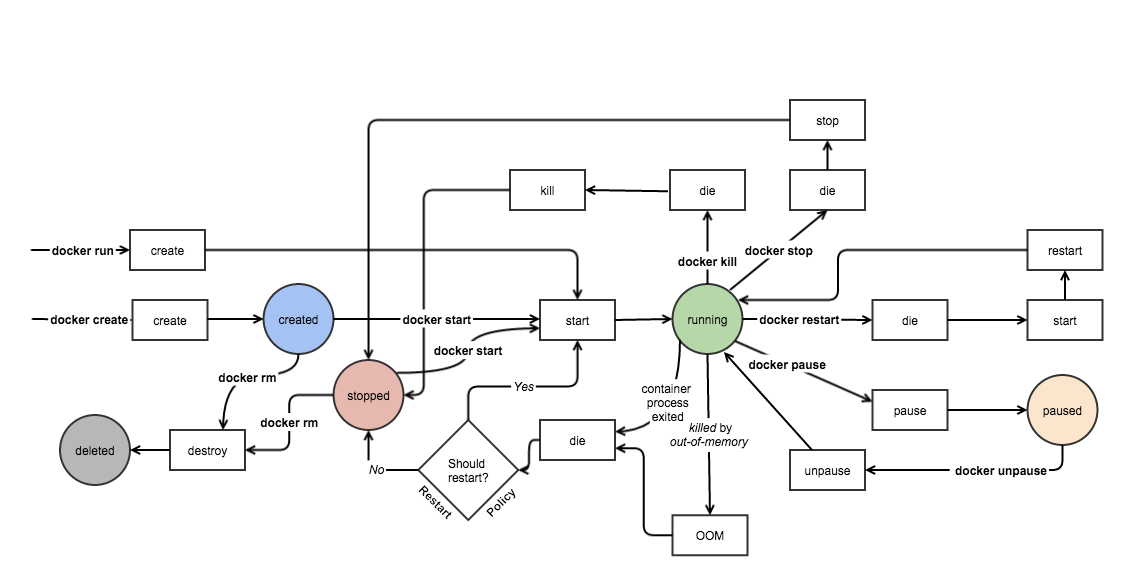
\includegraphics[width=\linewidth]{container_lifecycle.png}
                    \caption[Container Lifecycle]{Image portraying a \texttt{container}'s lifecycle. \cite{bib:container-lifecycle}}
                    \label{fig:container-lifecycle}
                \end{sidewaysfigure}

                We feel it is extremely important to draw the reader's attention to entry \ref{it:proc-death} in the enumeration describing a container's lifecycle. The fact that the exit of a container's main process effectively stops it implies that we can indeed stop containers through means not depending on the \texttt{docker stop} command. Given we are running an \texttt{ssh} daemon within the containers, we can log in as \texttt{root} and then issue \texttt{kill 1} to effectively stop the container. After all, \texttt{docker stop} will send the \texttt{SIGTERM} signal to the process running within the container and, should it not behave appropriately, \texttt{SIGKILL} after a configurable delay. Even though this subtlety will not impact the use we make of the virtual environments we are to work with it is a crucial aspect to bear in minf to fully understand the lifecylce of containers.\\

            \subsubsection{Container Capabilities}
                Due to the actions we want to perform inside our containers we need to provide them with some capabilities beyond the default ones. In the case of the regular nodes, we need to provide the \texttt{SYS\_ADMIN} capability so that they can change their own hostname with the \texttt{hostname} command. Routers will also need to be granted the \texttt{NET\_ADMIN} capability so that they can configure their own \texttt{iptables} rules. These capabilities are granted to containers when they are run thorough the \texttt{--cap-add} option.\\

                What is more, we need to allow the routers to forward packets through them. Besides instantiating the proper rules in \texttt{iptables} we also need to allow the \texttt{kernel} to process these packets. We can do so through the \texttt{--sysctl} option when running the container, thus enabling \texttt{ip forwarding} with the \texttt{net.ipv4.ip\_forward=1} parameter. This would be equivalent to running \texttt{\allowbreak echo 1 > /proc/sys/net/ipv4/ip\_forward} within an active container. The catch is that \texttt{/proc/sys} is mounted as \texttt{read-only} within containers. This would imply that we need to grant many more capabilities to said container so that we could run \texttt{mount -o remount rw /proc/sys} and then overwrite the option manually. We believe it is more elegant to just configure the options we need when starting the container and that is what we willl do.\\

                In any case, these options can be seen in the commands shown on listing \ref{lst:running-nodes}.\\

            \subsubsection{Docker's Internal Networks}
                The avid reader might have noticed how, after installing \texttt{docker} on an end system the output of the \texttt{ip addr} command within the machine has a different output: the \texttt{docker0} interfce is added as a gateway for the containers allowing them to reach the ``outside world''. What's more, after installing \texttt{docker} the \texttt{iptables} rules on the machine change as well. Running \texttt{iptables -L} shows a myriad of new \texttt{chains} with names such as \texttt{DOCKER-USER} and things along the lines of \texttt{DOCKER-ISOLATION-STAGE-*}. This approach to networking does simplify the issues one might run into when trying to make a ``normal'' use of a network, that is, when someone wants to either isolate a container from the external network or provide outwards connectivity. This is by no means our endeavour: we want to work with arbitrarily complex network topologies.\\

                In the realm of technology one often finds that simplifying the operation of a given software system implies making assumptions and avoiding exposing configuration parameters to the end user. Whilst this is a totally reasonable approach it is \textbf{not} one suited to us. This justifies the fact that we discarded the preexisting \texttt{docker network} model. This translates into us passing the \texttt{--network none} option to commands such as \texttt{docker run}, for instance. Just like when we discussed the role \texttt{kubernetes} plays when orchestrating containers, we feel it is pointless to use a tool only to go against it time and time again.\\

            \subsubsection{Our Approach}
                Our framework makes extensive use of the \texttt{docker run} command to both \texttt{create} and \texttt{start} the containers with the same action. The network topologies we are to set up contain a myriad of nodes, so allocating a \texttt{tty} for each of them makes handling things tremendously unwieldy. That is why we will always use the \texttt{-d} option, thus \texttt{detaching} the container. This translates into \texttt{docker} instantaneously returning control of the shell session we are currently using as soon as the container itself is up and running. What's more, we will also run the container with \textbf{no} network connections: remember we will manually set the entire networking infrastructure up. The commands we use to run both types of images, that for routers and nodes, is shown on listing \ref{lst:running-nodes}.\\

                \begin{lstlisting}[language = bash, caption = Running network nodes., label = lst:running-nodes]
                    # Running regular network nodes.
                    docker run -d --name <node-name> --network --cap-add SYS_ADMIN none ubuntu_node

                    # Running routers.
                    docker run -d --name <router-name> --network none --cap-add SYS_ADMIN --cap-add NET_ADMIN --sysctl net.ipv4.ip_forward=1 ubuntu_router
                \end{lstlisting}

                Running the container in the background poses the question of how we are to ``get inside the container'' to act as a regular user. In other words, how can we log into a \texttt{detached} container? Given \texttt{docker}'s architecture, and the fact that we are running an \texttt{SSH} daemon as the container's main process, we have two options to attain this result.\\

                \paragraph{Executing Commands Within the Container}
                    As shown in table \ref{tab:docker-commands}, we can always use the \texttt{docker exec} command to execute a command within a running container. If what we want to do is start a \texttt{bash} shell within the container (Ubuntu's default shell) we can just execute the command found on listing \ref{lst:docker-exec}. We can also take a look at the processes running within the container to confirm how \texttt{sshd}'s \texttt{PID} is indeed $1$ (it was the first process to spawn in the container). Aside from that process, we will only see the current \texttt{shell} session together with the \texttt{ps} program too. This approach can of course be leveraged to run single-non interactive commands within the containers. We could for instance run \texttt{docker exec <container-name> ps ax} to list a containers processes, for instance.\\

                    \begin{lstlisting}[language = bash, caption = Inspecting a container's processes., label = lst:docker-exec]
                        # Spawning our test container.
                        docker run -d --name test_node ubuntu_node

                        # Running a shell within it:
                            # -i: Interactive command (i.e. keep STDIN open).
                            # -t: Allocate a pseudo-TTY (i.e. a software
                                # emulated terminal).
                        docker exec -it test_node bash

                        # Listing the existing processes:
                            # a: Show all processes with an allocated TTY.
                            # x: Include processes without an allocated TTY.
                            # These two options effectively select every process.
                        ps ax

                        # Sample output:
                            # PID TTY      STAT   TIME COMMAND
                            # 1   ?        Ss     0:00 sshd: /usr/sbin/sshd -D \
                                # [listener] 0 of 10-100 startups
                            # 13  pts/0    Ss     0:00 bash
                            # 23  pts/0    R+     0:00 ps ax
                    \end{lstlisting}

                \paragraph{Logging in Through SSH}
                    We previously explained why our containers were going to run an \texttt{ssh} daemon as their main process. This not only ``keeps them alive'', but it also allows external connections to be made from the outside world. Thus, once we know the \texttt{IP} address associated to a given container we can log into it from the host running \texttt{docker} as long as we do have connectivity with the container itself. If we spawn a container using the same command as the one shown in listing \ref{lst:docker-exec} we can verify how it has been given an \texttt{IP} by the docker daemon with the command found on listing \ref{lst:checking-container-ip}. Then, we can just run \texttt{ssh root@<container-ip>} to log into that machine as we would normally do in any other system. The password is, of course, \texttt{1234} as specified in the \texttt{Dockerfiles} we used to build the images these containers will be running.\\

                    This aspect shows one of the great strengths of our approach when instantiating the entire networking infrastructure ourselves: we can choose whether to isolate the entire virtual scenario from the outside or not. This would permit or forbid an external user to log into our containers for instance. All we would have to do is add a \texttt{veth} connecting one of the virtual routers and the machine running the containers: as simple as that.\\

                    \begin{lstlisting}[language = bash, caption = Checking a container's \texttt{IP} address., label = lst:checking-container-ip]
                        docker inspect -f {{.NetworkSettings.IPAddress}}\
                            <container-name>
                    \end{lstlisting}

                \paragraph{Attaching to the Container}
                    We can theoretically leverage a third option: \texttt{attaching} a terminal session to the running container. This will \textbf{not} behave as we would expect however. In our case, attaching a shell to our container would make us ``see'' the \texttt{ssh} daemon we are running as the container's initial process. This would't allow us to perform any actions whatsoever: we wouldn't be attaching ourselves to an interactive process, so it is of very little use. We nonetheless felt it was worthwhile to mention this option did indeed exists: it might prove to be useful under different circumstances.\\

    The framework for instantiating virtual networks leverages the different technologies we have discussed throughout this chapter. The next one shows a ``toy example'' demonstrating the use of all of them to bring up a simple topology comprising two containers and a bridge mediating between them.\\
